\chapter{\gls{JPEG}}

\section{\gls{ITU} standard}
\begin{itemize}
\item Supported by all Web browsers, and most image viewers, define
  how to compress raster images \cite{ccitt.t81}.
\item Developed by the \gls{JPEG} (\href{https://www.itu.int}{ITU}),
  in 1992.
\end{itemize}
\vspace{-2ex}
\begin{center}
  \href{https://en.wikipedia.org/wiki/Magnetic_resonance_imaging_of_the_brain#/media/File:MRI_of_Human_Brain.jpg}{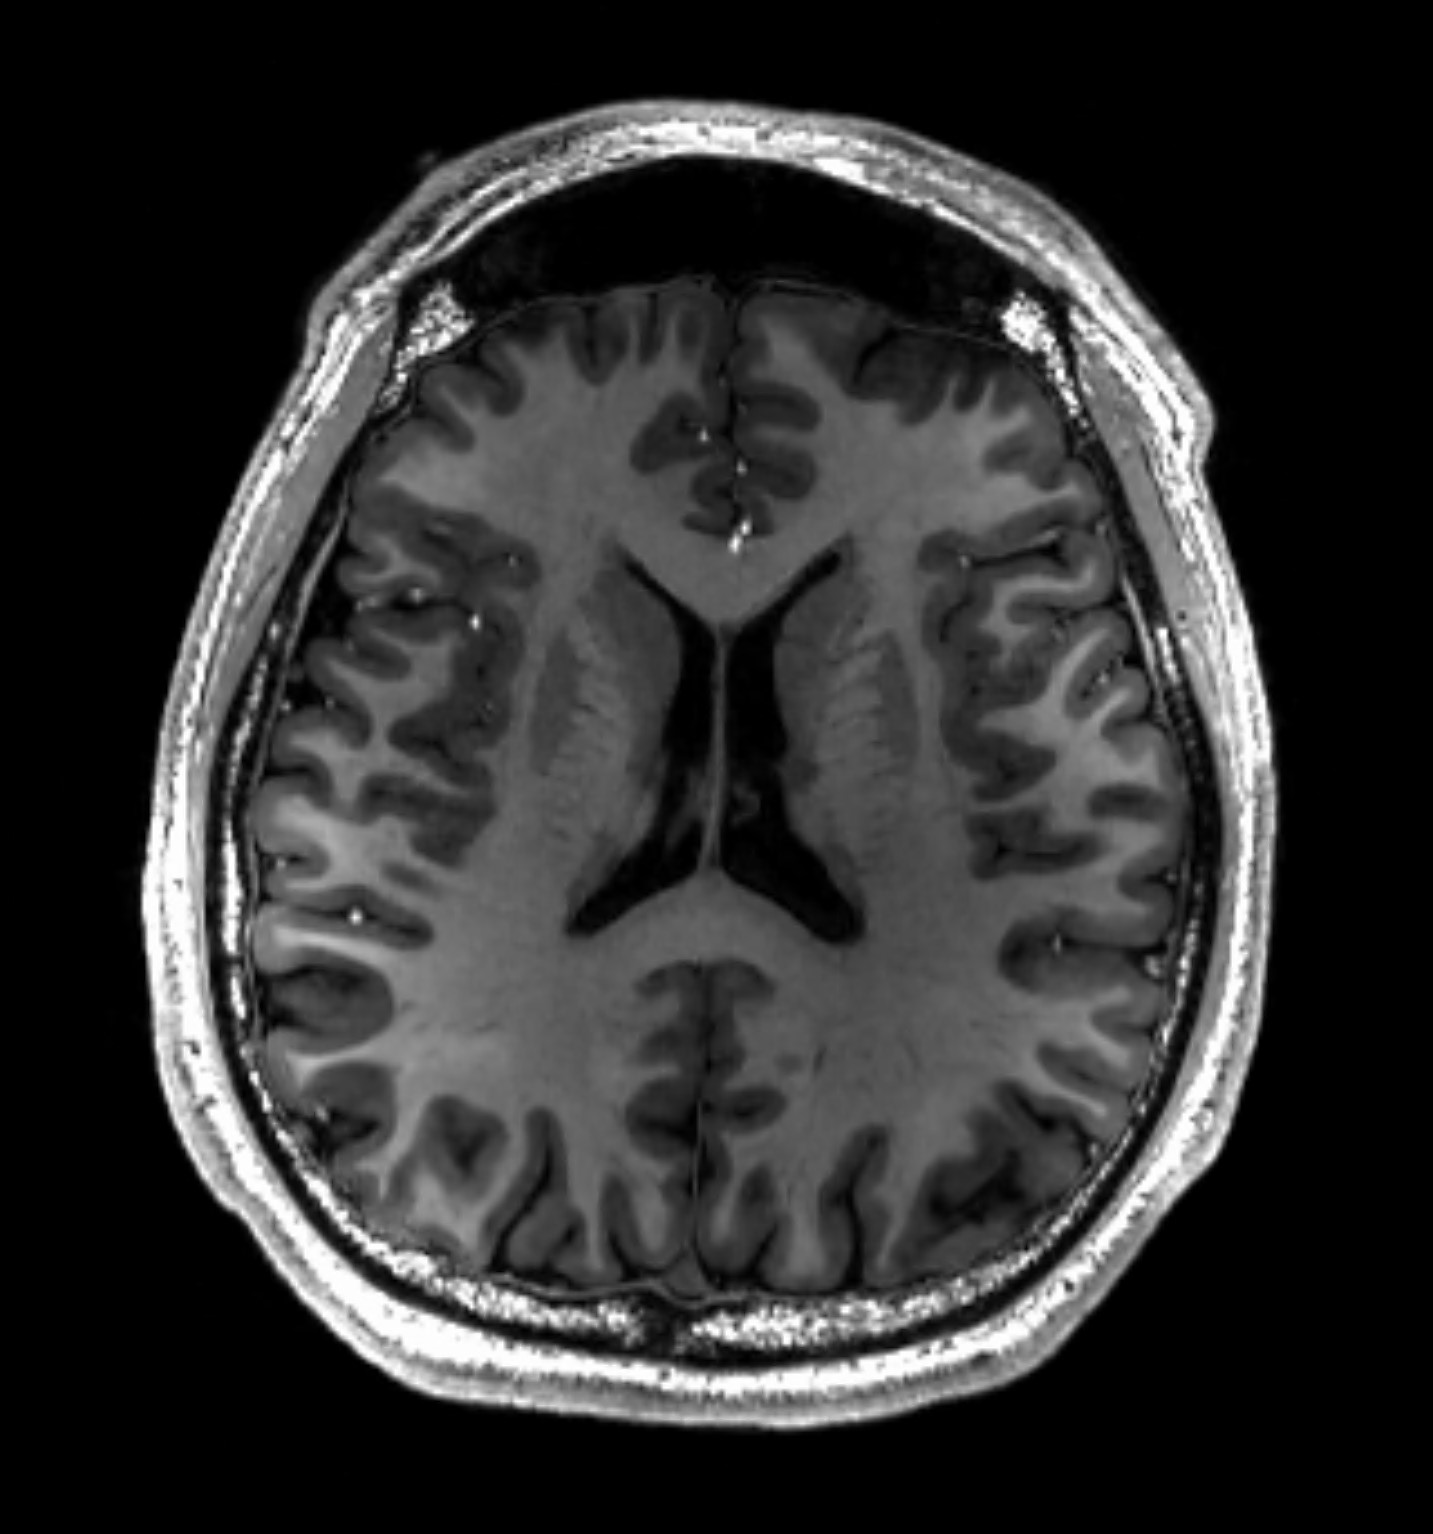
\includegraphics[width=4.0cm]{MRI_of_Human_Brain}}\\
  (click on the image)
\end{center}

\section{Lossy compression of color natural images}
\begin{itemize}
\item Designed for achieve high compression ratios, but at the expense of reducing quality.
  \item Raster images with up to ($2^{16}-1$)x($2^{16}-1$) pixels.
  \item Pixels must be gray-scale or \gls{RGB}, 8 bits/channel.
\end{itemize}
\vspace{-2ex}
\begin{center}
  \href{https://www.thewebmaster.com/jpeg-definitive-guide/}{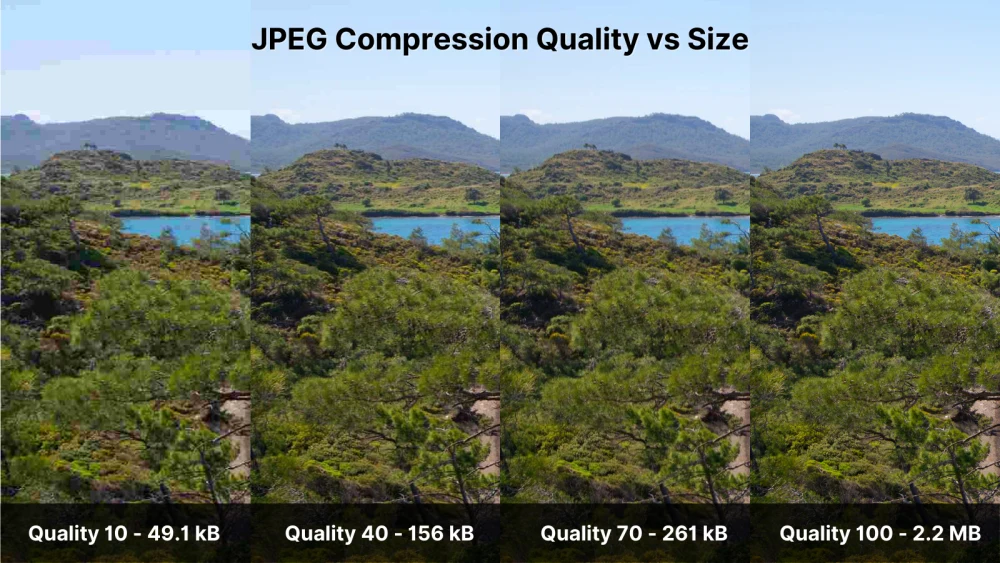
\includegraphics[width=8.5cm]{JPEG_Quality_vs_Size}}
\end{center}

\section{Algorithm}
\begin{enumerate}
\item Convert from the \gls{RGB} color space to the \gls{YCbCr} color
  space. Only if the input image is in color.
\item Subsample the crominance (Cr and Cb channels). /* Lossy step */
\item Divide each channel in blocks of size 8x8. \popup{The rest of
    steps work by blocks}{This makes it possible to work at the block
    level regardless of the image size.}.
\item Transform each block using the \gls{DCT}.
\item Quantize the \gls{DCT} coefficients. /* Lossy step */
\item Entropy encode the quantized coefficients.
\end{enumerate}

\section*{}
\begin{itemize}
\item A graphic description of a compression of a gray-scale image.
\end{itemize}
\vspace{-2ex}
\begin{center}
  \href{https://link.springer.com/article/10.1007/s40799-019-00358-4}{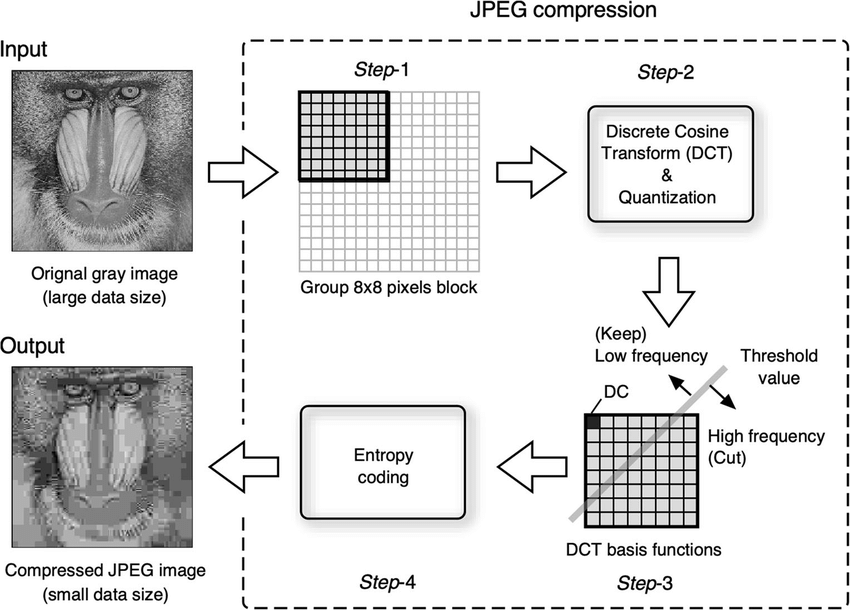
\includegraphics[width=8.5cm]{JPEG}}
\end{center}

\section{Artifacts}
\begin{itemize}
\item The human eye is sensitive to the 8x8-blockiness.
\end{itemize}
\vspace{-2ex}
\begin{center}
  \href{https://thesai.org/Publications/ViewPaper?Volume=6&Issue=4&Code=ijacsa&SerialNo=16}{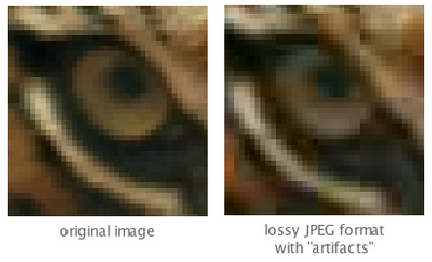
\includegraphics[width=10cm]{JPEG_blocking}}
\end{center}

\section{Progressive rendering}
\begin{itemize}
\item Optinal. Blocks are reconstructed coefficient-by-coefficient following the Zig-Zag ordering.
\item During a progressive visualization, blocks display higher
  spatial frequencies.
\end{itemize}
\begin{center}
  \href{https://es.m.wikipedia.org/wiki/Archivo:Zigzag_scanning.jpg}{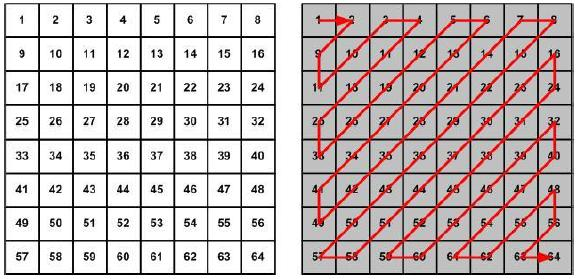
\includegraphics[width=8cm]{Zigzag_scanning}}
\end{center}

\section{Metadata}
\begin{itemize}
\item \gls{JPEG} images can store metadata as
  \href{https://en.wikipedia.org/wiki/Exif}{Exif} data (see the \href{https://gitlab.com/TNThieding/exif/-/blob/master/docs/api_reference.rst?ref_type=heads}{Exif implementation}). Some fields are:
  \vspace{-2ex}
  \begin{center}
    \begin{tabular}{l|l}
      Keyword & Meaning\\
      \hline
      ImageWidth & Width of the image in pixels \\
      ImageLength & Height of the image in pixels \\
      BitsPerSample&  Number of bits per color \\
      Make & Manufacturer of the camera or scanner \\
      Model & Model of the camera or scanner \\
      Software & Software used to process the image \\
      Orientation & Of the camera when the image was taken \\
      DateTimeOriginal & Date and time the image was originally captured \\
      ExposureTime & hutter speed \\
      FNumber & Lens aperture setting \\
      FocalLength & Focal length of the lens \\
      UserComment & User's comments about the image
    \end{tabular}
  \end{center}
\end{itemize}

\section*{}
\begin{itemize}
\item
  \href{https://github.com/vicente-gonzalez-ruiz/medical_imaging/blob/main/notebooks/JPEG_add_metadata.ipynb}{Here}
  there is an example that shows and modifies the metadata in a JPEG
  image.
\end{itemize}
